% !TEX program = xelatex
\documentclass[12pt,aspectratio=1610]{beamer}

% Presento style file
\usepackage{config/presentation}
%\usepackage[english]{babel}
\usepackage{booktabs}    
\usepackage{multirow}     
\usepackage{array}       
\usepackage[table]{xcolor} 
\usepackage{colortbl}
\definecolor{headbg}{HTML}{EEF2FF}
\definecolor{stubbg}{HTML}{F1F5F9}
\definecolor{rowA}{HTML}{FFFFFF}
\definecolor{rowB}{HTML}{F8FAFC}
\definecolor{rulecol}{HTML}{CBD5E1}
\usetikzlibrary{shapes.geometric,fit}
\newsavebox{\Hbox}
\newsavebox{\Honebox}
\newsavebox{\Htwobox}
\newsavebox{\Hthreebox}
%\arrayrulecolor{rulecol}          
\setlength{\tabcolsep}{8pt}       
\renewcommand{\arraystretch}{1.25}

% Information
\title{Performance paradoxes in matching systems are not that rare}
%\subtitle{A super-duper Beamer template for wonderful researchers}
\author{{\large Shu LI}\\[7mm] 
{\normalsize  Joint work with: Ana Bu\v{s}i\'{c}, Jean-Michel Fourneau and Antoine Lunven}}
\institute[INRIA]{
{
\large NETGCOOP 2025, Bilbao }}
\date{}



\begin{document}

% Title page
\begin{frame}[plain]
\maketitle
\end{frame}

\section{Introduction}
\begin{frame}{Stochastic Matching model}
\begin{block}{Stochastic Matching model, Mairesse \& Moyal, JAP, 2016 } 
A Matching model is  a triple $(G,\Phi,\alpha)$ defined by a non-bipartite matching graph $G=(\cal{V},\cal{E})$, a matching policy $\Phi$ and a distribution of probability $\alpha$ to model the arrivals of items.
\begin{itemize}
\item Items of the various classes in $\mathcal{V}$ arrive according to independent Poisson processes; their class i is drawn following $\alpha$ on $\mathcal{V}$.\\ 
\item Any incoming item is matched, if possible, with a compatible item present in the system; Otherwise it is stored in a buffer.\\ 
\item If several possible matches are possible, the incoming item follows a given matching policy $\Phi$, such as First Come First matched (FCFM).
\end{itemize}
\end{block}  
\end{frame}

\iffalse
\begin{frame}{Stochastic Matching model}
\begin{block}{Stochastic Matching model, Mairesse \& Moyal, JAP, 2016 }
A Matching model is  a triple $(G,\Phi,\alpha)$ defined by 
\begin{itemize}
\item a matching graph $G=(\cal{V},\cal{E})$ %which is an undirected graph 
whose nodes in $\cal{V}$ are classes of items 
and whose edges $\cal{E}$ in models the allowed matching of items. 
\item $\Phi$ is a matching policy.
\item a probability $\alpha$ on $\cal{V}$, the common law of the i.i.d. classes of the arriving items.
\end{itemize} 
The sequence of buffer-content forms a Markov chain. The stability problem consists of determining the conditions on $(G,\Phi,\alpha)$ for the Markov chain to be positive recurrent.
\end{block}  
\end{frame}\fi

\begin{frame}{NCOND}
The stability region of $(G, \Phi)$ is the set of probability measures $\alpha$ on $\mathcal{V}$ such that the natural Markov chain of $(G,\Phi,\alpha)$ is positive recurrent.
\begin{block}{NCOND}
A necessary condition of stability under the FCFM discipline  
that $\alpha(\mathcal{I})<\alpha(\Gamma(\mathcal{I}))$ for every independent set $\mathcal{I} $ in $\mathbb{I}$.
\end{block} 
\begin{figure}
\begin{minipage}{0.44\textwidth}
\begin{itemize}
\item $\mathcal{I}:=\{i| \{i,j\}\not\in\mathcal{E}\}\text{ for }\forall j\in\mathcal{I}\}$ 
\item  $\Gamma(\mathcal{I})=\{j|\{i,j\}\in\mathcal{E},i\in\mathcal{I}\}$
\end{itemize}
\end{minipage}
\hspace{3pt}
\begin{minipage}{0.53\textwidth}
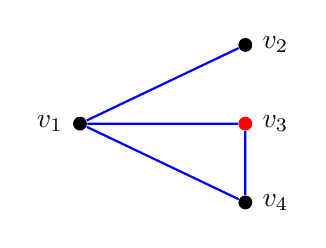
\begin{tikzpicture}[scale=1, vertex/.style={minimum width=5pt, circle, inner sep=0pt}]
\node[vertex,fill, label=left:$v_1$, xshift=-5.3cm, yshift=-3.5cm, anchor=north east] (1) at (current page.north east) {};
\node[vertex,fill, label=right:$v_2$, xshift=2.1cm, yshift=1.0cm] (2) at (1) {};
\node[vertex,fill=red, label=right:$v_3$, xshift=2.1cm, yshift=0.0cm] (3) at (1) {};
\node[vertex,fill, label=right:$v_4$, xshift=2.1cm, yshift=-1.0cm] (4) at (1) {};
%\draw[thick, red] (3) to [out=45, in=315, loop, min distance=1cm](3);
\draw[thick, blue](1)--(3)--(4)--(1)--(2);
\end{tikzpicture}
%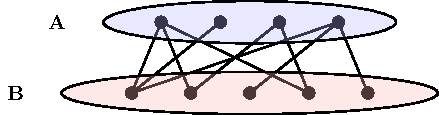
\includegraphics[width=0.8\linewidth]{images/biAB}
\end{minipage}
\end{figure}

%\begin{block}{Bipartite graph}
%Markov models associated with bipartite compatibility graphs cannot be ergodic. 
%\end{block} 
\end{frame}

\begin{frame}{Expectation}
	
{\color{blue}\small $E[G,\alpha]$ is the expected total number of items in the system at steady-state.} 
	
For all independent sets $\mathcal{I} \in \mathbb{I}$, consider an ordered version of $\mathcal{I}$ noted $\mathcal{I}^o=$ $\left\{i_1, \cdots, i_{|\mathcal{I}|}\right\}$, we note $\sigma$ a permutation of its elements, i.e $\mathcal{I}^{\sigma(o)}=\left\{i_{\sigma(1)}, \cdots, i_{\sigma(|\mathcal{I}|)}\right\}$ and $\mathfrak{S}_{|\mathcal{I}|}$ the set of all permutations on the nodes of $\mathcal{I}$. We define:
\[
T_{\mathcal{I}^o}=\prod_{k=1}^{|\mathcal{I}|} 
\frac{\alpha(\{i_k\})}
{ \alpha(\Gamma (\left\{i_1, \cdots, i_k\right\}))
-\alpha(\left\{i_1, \cdots, i_k\right\})}.
\]
Furthermore $T_{\mathcal{I}}=\sum_{\sigma \in \mathfrak{S}_{|\mathcal{I}|}} T_{\mathcal{I}^{\sigma(o)}}$.
We also define: 
\[
E_{\mathcal{I}^o}=\sum_{l=1}^{|\mathcal{I}|} 
\frac{\alpha(\Gamma(\{i_1, \cdots, i_l\})}{ \alpha(\Gamma( \{ i_1, \cdots, i_l \})) -\alpha(\{i_1, \cdots, i_l\})} \prod_{k=1}^{|\mathcal{I}|} \frac{\alpha(\{i_k\})}
{ \alpha(\Gamma( \{ i_1, \cdots, i_k \})) -\alpha(\{i_1, \cdots, i_k\})}
\]
Finally,  $E_{\mathcal{I}}=\sum_{\sigma \in \mathfrak{G}_{|\mathcal{I}|}} E_{\mathcal{I}^{\sigma(o)}}$. 
$\mathbb{E}[G, \alpha ]$  can be rewritten as 
\begin{equation}\label{eq:exceptio}
\mathbb{E}[G,\alpha]=\left(1+\sum_{\mathcal{I} \in \mathbb{I}}T_{\mathcal{I}}\right)^{-1}\left(\sum_{\mathcal{I}\in \mathbb{I}} E_{\mathcal{I}}\right)
\end{equation}
\end{frame}

\begin{frame}{Performance Paradox}

%{\color{purple} For some arrival rates $\alpha$, we define $\mathbb{E} [G, \alpha] $ as  the expection of the  total number of items in the system under FCFM.}
\begin{block}{Cadas, Doncel, Fourneau \& Busic. ACM SIGMETRICS, 2022}
For some arrival rates $\alpha$, we have a performance paradox 
if  $\mathbb{E} [G+e, \alpha]  > \mathbb{E} [G, \alpha]$. 
\end{block}

\begin{figure}[htbp]
\centering
\begin{minipage}{0.33\textwidth}
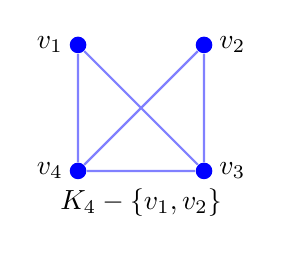
\begin{tikzpicture}[scale=0.8, vertex/.style={minimum width=6pt, circle,fill=blue, inner sep=0pt}]
\node[vertex](1)at(-1,1){};
\node[vertex](2)at(1,1){};
\node[vertex](3)at(1,-1){};
\node[vertex](4)at(-1,-1){};
\node[left=2pt] at (1){$v_1$};
\node[right=2pt] at (2){$v_2$};
\node[right=2pt] at (3){$v_3$};
\node[left=2pt] at (4){$v_4$};
\draw[blue!50,thick] (3) -- (1) -- (4) -- (3) -- (2) -- (4);
\node(c5) at (0,-1.5){$K_4-\{v_1,v_2\}$};
\end{tikzpicture}
\end{minipage}
\hspace{6pt}
\begin{minipage}{0.33\textwidth}
\centering
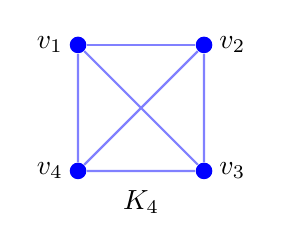
\begin{tikzpicture}[scale=0.8, vertex/.style={minimum width=6pt, circle, fill=blue, inner sep=0pt}]
\node[vertex](1)at(-1,1){};
\node[vertex](2)at(1,1){};
\node[vertex](3)at(1,-1){};
\node[vertex](4)at(-1,-1){};
\node[left=2pt] at (1){$v_1$};
\node[right=2pt] at (2){$v_2$};
\node[right=2pt] at (3){$v_3$};
\node[left=2pt] at (4){$v_4$};
\draw[blue!50,thick] (3) -- (1) -- (4) -- (3) -- (2) -- (4);
\draw[blue!50,thick]  (1) --  (2);
\node(c5) at (0,-1.5){$K_4$};
\end{tikzpicture}
\end{minipage}
\end{figure}

\begin{table}
\begin{tabular}{c|p{5cm}|p{5cm}}
\hline
\multirow{2}*{EX.1}& \multicolumn{2}{l}{\cellcolor{blue!10}$\alpha=(0.21, 0.21, 0.475, 0.105)$}\\
\cline{2-3}
&\cellcolor{blue!3}$\mathbb{E}[K_4-\{v_1,v_2\},\alpha]=8.252$ 
&\cellcolor{blue!3}$\mathbb{E}[K_4,\alpha]=8.883$\\
\hline
\end{tabular}
\end{table}
\end{frame}

\begin{frame}{Background}
\begin{fullpageitemize}
\item {\color{blue}A product form for the general stochastic matching model.\\ Moyal, Busic, and Jean Mairesse. JAP, 2021 }
\item {\color{red}Flexibility can hurt dynamic matching system performance.\\ Cadas, Doncel, Fourneau and Busic. ACM SIGMETRICS, 2022}
%\item \textbf{Conjecture:} Do all examples with paradox contain a star in the compatibility graph?
\item {\color{blue}A general stochastic matching model on multigraphs.\\ Begeot, Marcovici, Moyal and Rahme. LAJPMS, 2021.}
\item {\color{red}$\mathbb{E}[G,\alpha]$ for the multigraphs ?}
\end{fullpageitemize}
\end{frame}

\begin{frame}{Property}
%The union of simple graphs $G$ and $H$ is the graph $G \cup H$ with vertex set $\mathcal{V}(G)\cup\mathcal{V}(H)$ and edge set $\mathcal{E}(G)\cup \mathcal{E}(H)$.
Let $G1=(V1,E1) $ and  $G2=(V2,E2) $ two arbitrary graphs, 
the join of $G1$ and $G2$ (denoted as $G1 \bowtie G2$) is defined by the set of nodes $V1 \cup V2$ and the set 
of edges $E1 \cup E2 \cup V1 \times V2$, where $\times $ is the Cartesian product. 
%By starting with a disjoint union of two graphs $G$ and $H$  and adding edges joining every vertex of $G$ to every vertex of $H$, one obtains the join of $G$ and $H$, denoted $G \bowtie H$.
\begin{block}{Busic,Cadas,Doncel,Fourneau,Queueing Systems,2024}
Performance paradoxes exist for graphs $IN_n \bowtie (K_4 -(1,2)) $ where $ IN_n$ is the graph with $n$ isolated nodes. 
\end{block}
\begin{figure}
\begin{minipage}{0.34\textwidth}
{The join of $4$ isolated vertices and $K_4 -(1,2)$: $IN_4 \bowtie (K_4 -(1,2))$.}
\end{minipage}
\hspace{4pt}
\begin{minipage}{0.62\textwidth}
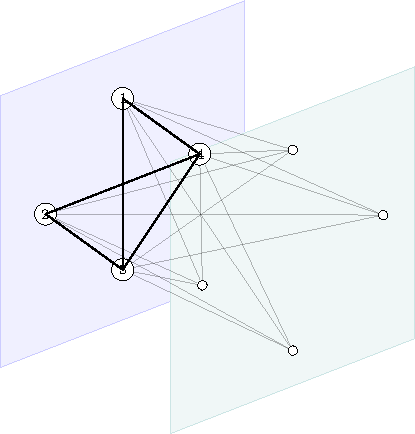
\includegraphics[width=0.52\linewidth]{images/IN4K4.pdf}
\end{minipage}
\end{figure}

\pause % 点击一下后再显示
\tikz[remember picture,overlay]{
\node at (current page.south) [yshift=2.3cm] {%
\begin{minipage}{0.90\paperwidth}
\begin{beamercolorbox}[wd=\linewidth,sep=4pt]{block title}
\usebeamerfont{block title}Conjecture
\end{beamercolorbox}
\vspace{-1pt}
\begin{beamercolorbox}[wd=\linewidth,sep=6pt]{block body}
\usebeamerfont{block body}All examples with paradox so far contain a star. Is it needed?
\end{beamercolorbox}
\end{minipage}};
}
\end{frame}

\section{Paradox in Star-free Graphs}

\begin{frame}{The Minimal odd unicycle}

% ------- 图形宏（复用，与你的 TikZ 相同） -------
\newcommand{\Cfive}{%
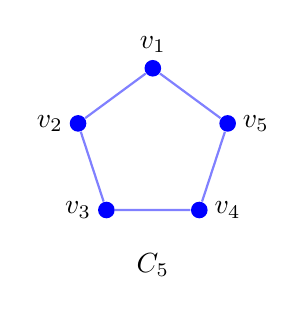
\begin{tikzpicture}[scale=1, vertex/.style={minimum width=6pt, circle,fill=blue, inner sep=0pt}]
\foreach \i/\x/\y in {1/0/1, 2/0.95/0.3, 3/0.59/-0.8, 4/-0.59/-0.8, 5/-0.95/0.3}
\node[vertex] (v\i) at (\x,\y) {};
\node[above=2pt] at (v1){$v_1$};
\node[right=2pt] at (v2){$v_5$};
\node[right=2pt] at (v3){$v_4$};
\node[left=2pt]  at (v4){$v_3$};
\node[left=2pt]  at (v5){$v_2$};
\draw[blue!50,thick] (v1)--(v2)--(v3)--(v4)--(v5)--(v1);
\node at (0,-1.5){$C_5$};
\end{tikzpicture}
}

\newcommand{\Fone}{%
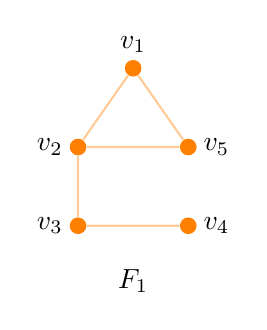
\begin{tikzpicture}[scale=1, vertex/.style={minimum width=6pt, circle, fill=orange, inner sep=0pt}]
\node[vertex] (z1) at (0,1){};  \node[above=2pt] at (z1) {$v_1$};
\node[vertex] (z2) at (-0.7,0){}; \node[left=2pt]  at (z2) {$v_2$};
\node[vertex] (z3) at (-0.7,-1){};\node[left=2pt]  at (z3) {$v_3$};
\node[vertex] (z4) at (0.7,-1){}; \node[right=2pt] at (z4) {$v_4$};
\node[vertex] (z5) at (0.7,0){};  \node[right=2pt] at (z5) {$v_5$};
\draw[orange!40,thick](z2)--(z5)--(z1)--(z2)--(z3)--(z4);
\node at (0,-1.7){$F_1$};
\end{tikzpicture}
}

\newcommand{\Ftwo}{%
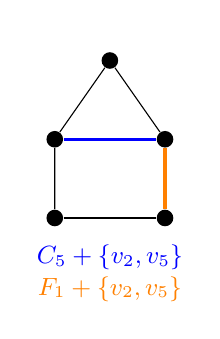
\begin{tikzpicture}[scale=1, vertex/.style={minimum width=6pt, circle, fill=black, inner sep=0pt}]
\node[vertex] (z1) at (0,1){};   \node[above=5pt] at (z1) {};
\node[vertex] (z2) at (-0.7,0){}; \node[vertex] (z3) at (-0.7,-1){};
\node[vertex] (z4) at (0.7,-1){}; \node[vertex] (z5) at (0.7,0){};
\draw (z5)--(z1)--(z2)--(z3);
\draw[blue, very thick](z2)--(z5);
\draw (z3)--(z4);
\draw[orange,very thick](z4)--(z5);
\node at (0,-1.5){{\small\color{blue}$C_5+\{v_2,v_5\}$}};
\node at (0,-1.9){{\small\color{orange}$F_1+\{v_2,v_5\}$}};
\end{tikzpicture}
}

% ------- 表格两段（EX.1 / EX.2） -------
\newcommand{\TableEXone}{%
\begin{tabular}{c|p{5cm}|p{5cm}}
\hline
\multirow{2}{*}{\textbf{EX.1}} &
\multicolumn{2}{l}{\cellcolor{blue!10}$\lambda=(0.111, 0.10575, 0.179426, 0.35046, 0.253364)$}\\
\cline{2-3}
&\cellcolor{blue!3}$\mathbb{E}[C_5,\lambda]=7.86$
&\cellcolor{blue!3}$\mathbb{E}[C_5+\{v_2,v_5\},\lambda]=8.17$\\

\hline
\end{tabular}
}

\newcommand{\TableEXtwo}{%
\begin{tabular}{c|p{5cm}|p{5cm}}
\hline
\multirow{2}{*}{\textbf{EX.2}} &
\multicolumn{2}{l}{\cellcolor{orange!10}$\lambda=(0.266025, 0.11005, 0.210855, 0.14145, 0.27162)$}\\
\cline{2-3}
&\cellcolor{orange!5}$\mathbb{E}[F_1,\lambda]=16.069$
&\cellcolor{orange!5}$\mathbb{E}[F_1+\{v_2,v_5\},\lambda]=16.89$\\
\hline
\end{tabular}
}

% ================= 三步切换 =================
% 步骤1：全部显示
\only<1>{
  \centering
  \begin{table}\begin{tabular}{c|p{5cm}|p{5cm}}
  \hline
  \multirow{2}{*}{\textbf{EX.1}} &
  \multicolumn{2}{l}{\cellcolor{blue!10}$\lambda=(0.111, 0.10575, 0.179426, 0.35046, 0.253364)$}\\
  \cline{2-3}
  &\cellcolor{blue!3}$\mathbb{E}[C_5,\lambda]=7.86$
  &\cellcolor{blue!3}$\mathbb{E}[C_5+\{v_2,v_5\},\lambda]=8.17$\\
  \hline
  \multirow{2}{*}{\textbf{EX.2}} &
  \multicolumn{2}{l}{\cellcolor{orange!10}$\lambda=(0.266025, 0.11005, 0.210855, 0.14145, 0.27162)$}\\
  \cline{2-3}
  &\cellcolor{orange!5}$\mathbb{E}[F_1,\lambda]=16.069$
  &\cellcolor{orange!5}$\mathbb{E}[F_1+\{v_2,v_5\},\lambda]=16.89$\\
  \hline
  \end{tabular}\end{table}

\begin{figure}\centering
\begin{minipage}{0.23\textwidth}\Cfive\end{minipage}\hspace{3pt}
\begin{minipage}{0.23\textwidth}\Fone \end{minipage}\hspace{3pt}
\begin{minipage}{0.23\textwidth}\Ftwo \end{minipage}
\caption{Graphs: $C_5$, $F_1$ and $C_5+\{v_2,v_5\}$ (or $F_1+\{v_2,v_5\}$).}
\end{figure}
}

% 步骤2：表格前两行 + 图1和图3
\only<2>{
  \centering
  \begin{table}\TableEXone\end{table}
  \begin{figure}\centering
    \begin{minipage}{0.23\textwidth}\Cfive\end{minipage}\hspace{3pt}
    \begin{minipage}{0.23\textwidth}\vspace*{2.5cm}\end{minipage}\hspace{3pt}% 占位，保持布局
    \begin{minipage}{0.23\textwidth}\Ftwo\end{minipage}
    \caption{Graphs: $C_5$ and $C_5+\{v_2,v_5\}$.}
  \end{figure}
}

% 步骤3：表格后两行 + 图2和图3
\only<3>{
\centering
\begin{table}\TableEXtwo\end{table}
\begin{figure}\centering
\begin{minipage}{0.23\textwidth}\vspace*{2.5cm}\end{minipage}\hspace{3pt}% 占位
\begin{minipage}{0.23\textwidth}\Fone\end{minipage}\hspace{3pt}
\begin{minipage}{0.23\textwidth}\Ftwo\end{minipage}
\caption{Graphs: $F_1$ and $F_1+\{v_2,v_5\}$.}
\end{figure}
}
\end{frame}

\iffalse
\begin{frame}{The Minimal odd unicycle}
\begin{table}
\begin{tabular}{c|p{5cm}|p{5cm}}
\hline
\multirow{2}*{EX.1}& \multicolumn{2}{l}{\cellcolor{blue!10}$\lambda=(0.111, 0.10575, 0.179426, 0.35046, 0.253364)$}\\
\cline{2-3}
&\cellcolor{blue!3}$\mathbb{E}[C_5,\lambda]=7.86$ 
&\cellcolor{blue!3}$\mathbb{E}[C_5,\lambda]=8.17$\\
\hline
\multirow{2}*{EX.2}
&\multicolumn{2}{l}{\cellcolor{orange!10}$\lambda=(0.266025, 0.11005, 0.210855,
0.14145, 0.27162)$}\\
\cline{2-3}
&\cellcolor{orange!5}$\mathbb{E}[F_1,\lambda]=16.069$
&\cellcolor{orange!5}$\mathbb{E}[F_2,\lambda]=16.89$\\
\hline
\end{tabular}
\end{table}

\begin{figure}[htbp]
\centering
\begin{minipage}{0.23\textwidth}
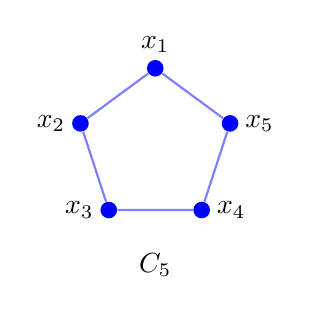
\begin{tikzpicture}[scale=1, vertex/.style={minimum width=6pt, circle,fill=blue, inner sep=0pt}]
\foreach \i/\x/\y in {1/0/1, 2/0.95/0.3, 3/0.59/-0.8, 4/-0.59/-0.8, 5/-0.95/0.3} {
\node[vertex] (v\i) at (\x,\y) {};
}
\node[above=2pt] at (v1){$x_1$};
\node[right=2pt] at (v2){$x_5$};
\node[right=2pt] at (v3){$x_4$};
\node[left=2pt] at (v4){$x_3$};
\node[left=2pt] at (v5){$x_2$};
\draw[blue!50,thick] (v1) -- (v2) -- (v3) -- (v4) -- (v5) -- (v1);
\node(c5) at (0,-1.5){$C_5$};
\end{tikzpicture}
\end{minipage}\hspace{3pt}
\begin{minipage}{0.23\textwidth}
\centering
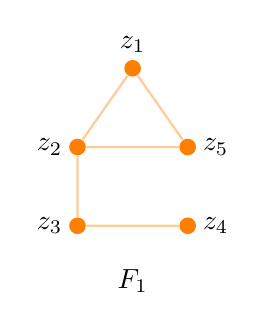
\begin{tikzpicture}[scale=1, vertex/.style={minimum width=6pt, circle, fill=orange, inner sep=0pt}]
\node[vertex] (z1) at (0,1){};
\node[above=2pt] at (z1) {$z_1$};
\node[vertex] (z2) at (-0.7,0){};
\node[left=2pt] at (z2) {$z_2$};
\node[vertex] (z3) at (-0.7,-1){};
\node[left=2pt] at (z3) {$z_3$};
\node[vertex] (z4) at (0.7,-1){};
\node[right=2pt] at (z4) {$z_4$};
\node[vertex] (z5) at (0.7,0){};
\node[right=2pt] at (z5) {$z_5$};
\draw[orange!40,thick](z2)--(z5)--(z1)--(z2)--(z3)--(z4);
\node at (0,-1.7){$F_1$};
\end{tikzpicture}
\end{minipage}\hspace{3pt}
\begin{minipage}{0.23\textwidth}
\centering
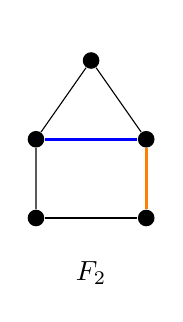
\begin{tikzpicture}[scale=1, vertex/.style={minimum width=6pt, circle, fill=black, inner sep=0pt}]
\node[vertex] (z1) at (0,1){};
\node[above=5pt] at (z1) {};
\node[vertex] (z2) at (-0.7,0){};
\node[vertex] (z3) at (-0.7,-1){};
\node[vertex] (z4) at (0.7,-1){};
\node[vertex] (z5) at (0.7,0){};
\draw (z5)--(z1)--(z2)--(z3);
\draw[blue, very thick](z2)--(z5);
\draw[](z3)--(z4);
\draw[orange,very thick](z4)--(z5);
\node at (0,-1.7){$F_2$};
\end{tikzpicture}
\end{minipage}
\caption{Graphs: $C_5$, $F_1$ and $F_2$ .}
\label{fig:twoc5}
\end{figure}
\end{frame}
\fi

\begin{frame}{A Star-Free Graph with Two Odd Cycles}
\begin{table}
\begin{tabular}{p{5cm}|p{5cm}}
\hline
\multicolumn{2}{l}{\cellcolor{blue!10}$\lambda=(0.231787, 0.462366, 0.14472, 0.127484, 0.00342, 0.030223)$}\\
\hline
\cellcolor{blue!3}$\mathbb{E}[F_3,\lambda]=31.59$ 
&\cellcolor{blue!3}$\mathbb{E}[F_3+\{v_1,v_5\},\lambda]=31.71$\\
\hline
\end{tabular}
\end{table}

\begin{figure}[htbp]
\centering
\begin{minipage}{0.5\textwidth}
\centering
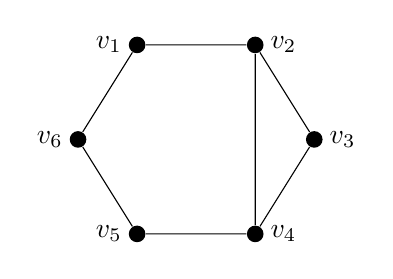
\begin{tikzpicture}[scale=1.5, vertex/.style={minimum width=6pt, circle, fill=black, inner sep=0pt}]
\node[vertex](v1) at (-0.5,0.8){};
\node[left=2pt] at (v1){$v_1$};
\node[vertex](v2) at (0.5,0.8){};
\node[right=2pt] at (v2){$v_2$};
\node[vertex](v3) at (1,0){};
\node[right=2pt] at (v3){$v_3$};
\node[vertex](v4) at (0.5,-0.8){};
\node[right=2pt] at (v4){$v_4$};
\node[vertex](v5) at (-0.5,-0.8){};
\node[left=2pt] at (v5){$v_5$};
\node[vertex](v6) at (-1,0){};
\node[left=2pt] at (v6){$v_6$};
\draw (v1)--(v2)--(v3)--(v4)--(v5)--(v6)--(v1);
\draw(v2)--(v4);
\end{tikzpicture}
\end{minipage}
\hspace{3pt}
\begin{minipage}{0.4\textwidth}
\centering
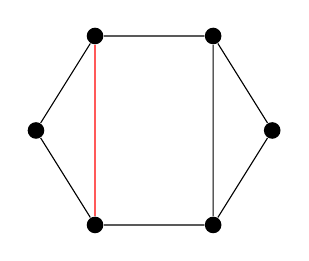
\begin{tikzpicture}[scale=1.5, vertex/.style={minimum width=6pt, circle, fill=black, inner sep=0pt}]
\node[vertex](v1) at (-0.5,0.8){};
\node[vertex](v2) at (0.5,0.8){};
\node[vertex](v3) at (1,0){};
\node[vertex](v4) at (0.5,-0.8){};
\node[vertex](v5) at (-0.5,-0.8){};
\node[vertex](v6) at (-1,0){};
\draw (v1)--(v2)--(v3)--(v4)--(v5)--(v6)--(v1);
\draw(v2)--(v4);
\draw[red](v1)--(v5);
\end{tikzpicture}
\end{minipage}
\caption{$F_3$ and $F_3+\{v_1,v_5\}$. }
\label{fig:twocycle}
\end{figure}
\end{frame}

\begin{frame}{$C_7$}
\begin{table}
\begin{tabular}{p{5cm}|p{5cm}}
\hline
\multicolumn{2}{l}{\cellcolor{blue!10}$\lambda=({0.045206, 0.240384, 0.303789, 0.146114, 0.132526, 0.111772, 0.020209})$}\\
\hline
\cellcolor{blue!3}$\mathbb{E}[C_7,\lambda]=129.56$ 
&\cellcolor{blue!3}$\mathbb{E}[C_7+\{v_1,v_5\},\lambda]=137.87$\\
\hline
\end{tabular}
\end{table}

\begin{figure}[htbp]
\centering
\begin{minipage}{0.4\textwidth}
\centering
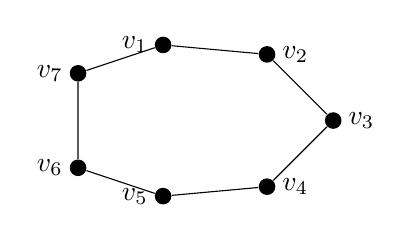
\begin{tikzpicture}[scale=1.2, vertex/.style={minimum width=6pt, circle, fill=black, inner sep=0pt}]
\node[vertex](v1) at (-0.5,0.8){};
\node[left=2pt] at (v1){$v_1$};
\node[vertex](v2) at (0.6,0.7){};
\node[right=2pt] at (v2){$v_2$};
\node[vertex](v3) at (1.3,0){};
\node[right=2pt] at (v3){$v_3$};
\node[vertex](v4) at (0.6,-0.7){};
\node[right=2pt] at (v4){$v_4$};
\node[vertex](v5) at (-0.5,-0.8){};
\node[left=2pt] at (v5){$v_5$};
\node[vertex](v6) at (-1.4,-0.5){};
\node[left=2pt] at (v6){$v_6$};
\node[vertex](v7) at (-1.4,0.5){};
\node[left=2pt] at (v7){$v_7$};
\draw (v1)--(v2)--(v3)--(v4)--(v5)--(v6)--(v7)--(v1);
\end{tikzpicture}
\end{minipage}
\hspace{3pt}
\begin{minipage}{0.4\textwidth}
\centering
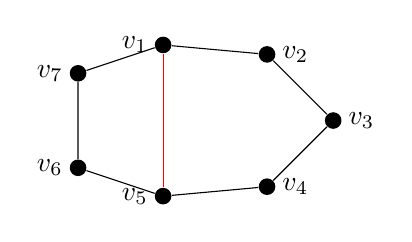
\begin{tikzpicture}[scale=1.2, vertex/.style={minimum width=6pt, circle, fill=black, inner sep=0pt}]
\node[vertex](v1) at (-0.5,0.8){};
\node[left=2pt] at (v1){$v_1$};
\node[vertex](v2) at (0.6,0.7){};
\node[right=2pt] at (v2){$v_2$};
\node[vertex](v3) at (1.3,0){};
\node[right=2pt] at (v3){$v_3$};
\node[vertex](v4) at (0.6,-0.7){};
\node[right=2pt] at (v4){$v_4$};
\node[vertex](v5) at (-0.5,-0.8){};
\node[left=2pt] at (v5){$v_5$};
\node[vertex](v6) at (-1.4,-0.5){};
\node[left=2pt] at (v6){$v_6$};
\node[vertex](v7) at (-1.4,0.5){};
\node[left=2pt] at (v7){$v_7$};
\draw (v1)--(v2)--(v3)--(v4)--(v5)--(v6)--(v7)--(v1);
\draw[red](v1)--(v5);
\end{tikzpicture}
\end{minipage}
\caption{$C_7$ and $C_7+\{v_1,v_5\}$. \label{fig:cycle7}}
\end{figure}
\end{frame}

\section{(Multi)-Graph with self loops} 
\begin{frame}{Definitions}
\begin{fullpageitemize}
\item $G=(\mathcal{V}, \mathcal{E})$: a multigraph with the nodes partition $\mathcal{V}=\mathcal{V}_1\cup\mathcal{V}_2$
\item {\color{blue}$\mathcal{V}_1=\{i\in \mathcal{V}\mid \{i,i\}\in \mathcal{E}\}$} and $\mathcal{V}_2 = \mathcal{V}\setminus \mathcal{V}_1$
\item $\check{G}=(\mathcal{V},{\color{orange}\mathcal{E}\setminus\{(i,i)\mid i\in\mathcal{V}_1\}})$
\item $\mathbb{I} (\check{G})$: the family of independent sets of $\check{G}$
\item $\mathcal{I}^o=\{e_1,\dots,e_{|\mathcal{I}|}\}$: an arbitrary ordering $\mathcal{I}\in\mathbb{I}(\check G)$
\item $\mathcal{I}^{\sigma(o)}=\{e_{\sigma(1)},\dots,e_{\sigma(|\mathcal{I}|)}\}$: the sequence obtained by applying 
$\sigma$ to the ordered version $\mathcal{I}^o$
\item $\mathcal{I}_k^o$: the first $k$ elements of $\mathcal{I}^o$
\item $\mathcal{J}_k^o=\mathcal{I}_k^o\cap \mathcal{V}_2$
\end{fullpageitemize}
\begin{tikzpicture}[remember picture, overlay,scale=1, vertex/.style={minimum width=5pt, circle, inner sep=0pt}]
\node[vertex,fill, label=left:$v_1$, xshift=-5.3cm, yshift=-3.5cm, anchor=north east] (1) at (current page.north east) {};
\node[vertex,fill, label=right:$v_2$, xshift=2.1cm, yshift=1.0cm] (2) at (1) {};
\node[vertex,fill=blue, label=right:$v_3$, xshift=2.1cm, yshift=0.0cm] (3) at (1) {};
\node[vertex,fill, label=right:$v_4$, xshift=2.1cm, yshift=-1.0cm] (4) at (1) {};
\draw[thick, red] (3) to [out=45, in=315, loop, min distance=1cm](3);
\draw[thick, orange](1)--(3)--(4)--(1)--(2);
\end{tikzpicture}
\end{frame}

\begin{frame}{Theorem}
We define 
$$
T_{\mathcal{I}^o}=\prod_{k=1}^{|\mathcal{I}|}\frac{\alpha(e_{k})}{\alpha\Bigl(\Gamma\bigl(\mathcal{I}_k^o\bigr)\Bigr)-\alpha\Bigl(\mathcal{J}_k^o\Bigr)},
$$
and $T_{\mathcal{I}}=\sum_{\sigma \in \mathfrak{S}_{|\mathcal{I}|}} T_{\mathcal{I}^{\sigma(o)}}$. Thus $\pi(\emptyset) = (1 +T_{\mathcal{I}})^{-1}$. 
We also define
$$E_{\mathcal{I}^o}=\sum_{l=1}^{|\mathcal{I}|}
\frac{\alpha\Bigl(\Gamma\bigl(\mathcal{I}_l^o\bigr)\Bigr)}
{\alpha\Bigl(\Gamma\bigl(\mathcal{I}_l^o\bigr)\Bigr)-
\alpha\Bigl(\mathcal{J}_l^o\Bigr)}\prod_{k=1}^{|\mathcal{I}|}\frac{\alpha(e_{k})}{\alpha\Bigl(\Gamma\bigl(\mathcal{I}_k^o\bigr)\Bigr)-
\alpha\Bigl(\mathcal{J}_k^o\Bigr)},$$
and $E_{\mathcal{I}}=\sum_{\sigma \in \mathfrak{S}_{|\mathcal{I}|}} E_{\mathcal{I}^{\sigma(o)}}$.
The expected number of items in steady state is
\begin{equation}\label{eq:exp-multi}
\mathbb{E}[G,\alpha]=\Bigl(1+\sum_{\mathcal{I}\in\mathbb{I}(\check G)}T_\mathcal{I}\Bigr)^{-1}\sum_{\mathcal{I}\in\mathbb{I}(\check G)}E_\mathcal{I}.
\end{equation}
\end{frame}

\begin{frame}{Corollary}
\begin{figure}
\centering
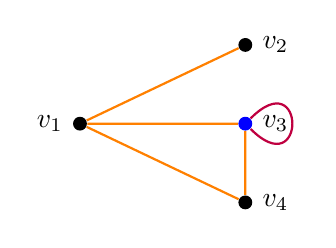
\begin{tikzpicture}[scale=1, vertex/.style={minimum width=5pt, circle, inner sep=0pt}]
\node[vertex,fill, label=left:$v_1$] (1) at (0,0) {};
\node[vertex,fill, label=right:$v_2$, xshift=2.1cm, yshift=1.0cm] (2) at (1) {};
\node[vertex,fill=blue, label=right:$v_3$, xshift=2.1cm, yshift=0.0cm] (3) at (1) {};
\node[vertex,fill, label=right:$v_4$, xshift=2.1cm, yshift=-1.0cm] (4) at (1) {};
\draw[thick, purple] (3) to [out=45, in=315, loop, min distance=1cm](3);
\draw[thick, orange](1)--(3)--(4)--(1)--(2);
\end{tikzpicture}
\hspace{10pt}
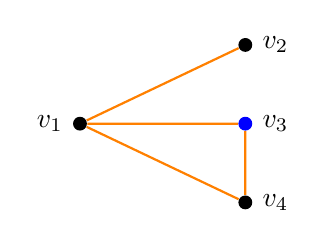
\begin{tikzpicture}[scale=1, vertex/.style={minimum width=5pt, circle, inner sep=0pt}]
\node[vertex,fill, label=left:$v_1$] (1) at (0,0) {};
\node[vertex,fill, label=right:$v_2$, xshift=2.1cm, yshift=1.0cm] (2) at (1) {};
\node[vertex,fill=blue, label=right:$v_3$, xshift=2.1cm, yshift=0.0cm] (3) at (1) {};
\node[vertex,fill, label=right:$v_4$, xshift=2.1cm, yshift=-1.0cm] (4) at (1) {};
\draw[thick, orange](1)--(3)--(4)--(1)--(2);
\end{tikzpicture}
\end{figure}
\begin{block}{For simple graph.Cadas, Doncel, Fourneau,Busic. 2022}
If $\mathcal{V}_1=\emptyset$,  then  $\mathcal{J}_k^o=\mathcal{I}_k^o$. 
\end{block}
\end{frame}

\begin{frame}{Tools and Examples}
\begin{tikzpicture}[remember picture, overlay, vertex/.style={minimum width=6pt, circle, inner sep=0pt}]
\coordinate (o) at (current page.west);
\node[xshift=3.3cm, yshift=3.3cm, anchor=north east] (github) at (o){
\includegraphics[width=1.3cm]{images/github.png}};
\node[xshift=0cm, yshift=-0.9cm] (python) at (github.south){
\includegraphics[width=1.3cm]{images/python.png}};
\node[xshift=0cm, yshift=-0.8cm] (myname) at (python.south){
\includegraphics[width=1.3cm]{images/myname.png}}; 
\node[xshift=1.3cm, yshift=0.5cm, anchor=north west] (gg2) at (github.north east){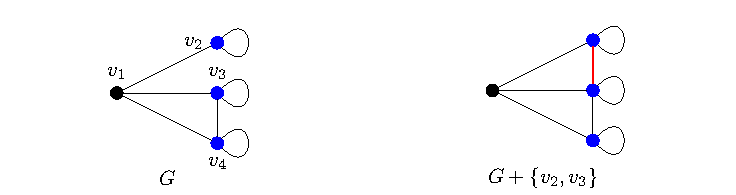
\includegraphics[width=10.0cm]{images/gg2.pdf}};
\node[xshift=0cm, yshift=-0.2cm, anchor=north west] (gcm) at (gg2.south west){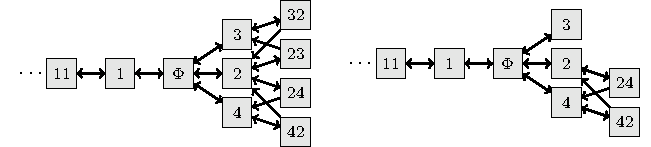
\includegraphics[width=9.0cm]{images/gcm.pdf}};
\node[xshift=0.4cm, yshift=-4.5cm, anchor=west] (table) at (github.south west){\begin{tabular}{p{5cm}|p{5cm}}
\hline
\multicolumn{2}{l}{\cellcolor{blue!10}$\lambda=(0.432685, 0.005861, 0.141128, 0.420326)$}\\
\hline
\cellcolor{blue!3}$\mathbb{E}[G,\lambda]=2.944793$ 
&\cellcolor{blue!3}$\mathbb{E}[G_2,\lambda]=2.947256$\\
\hline
\end{tabular}};
\end{tikzpicture}
\end{frame}

\begin{frame}{Examples}

\sbox{\Hbox}{%
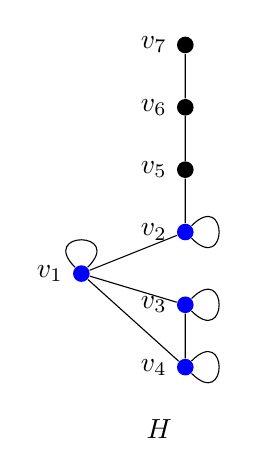
\begin{tikzpicture}[scale=0.66, vertex/.style={minimum width=6pt, circle, inner sep=0pt}]
\node[vertex,fill=blue, label=left:$v_1$](1) at (-1,0){};
\node[vertex,fill=blue, label=left:$v_2$](2) at (1,0.8){};
\node[vertex,fill=blue, label=left:$v_3$](3) at (1,-0.6){};
\node[vertex,fill=blue, label=left:$v_4$](4) at (1,-1.8){};
\node[vertex,fill, label=left:$v_5$](5) at (1,2){};
\node[vertex,fill, label=left:$v_6$](6) at (1,3.2){};
\node[vertex,fill, label=left:$v_7$](7) at (1,4.4){};
\draw (1) to [out=45, in=135, loop, min distance=1cm](1);
\draw (2) to [out=45, in=315, loop, min distance=1cm](2);
\draw (3) to [out=45, in=315, loop, min distance=1cm](3);
\draw (4) to [out=45, in=315, loop, min distance=1cm](4);
\draw(1)--(3)--(4)--(1)--(2)--(5)--(6)--(7);
\node at (0.5,-3){$H$};
\end{tikzpicture}}

\sbox{\Honebox}{%
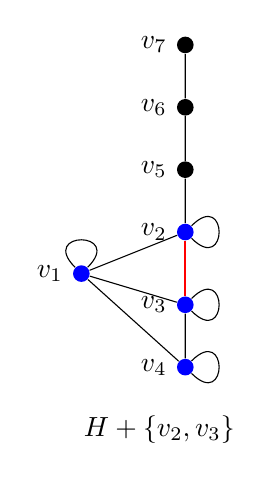
\begin{tikzpicture}[scale=0.66, vertex/.style={minimum width=6pt, circle, inner sep=0pt}]
\node[vertex,fill=blue, label=left:$v_1$](1) at (-1,0){};
\node[vertex,fill=blue, label=left:$v_2$](2) at (1,0.8){};
\node[vertex,fill=blue, label=left:$v_3$](3) at (1,-0.6){};
\node[vertex,fill=blue, label=left:$v_4$](4) at (1,-1.8){};
\node[vertex,fill, label=left:$v_5$](5) at (1,2){};
\node[vertex,fill, label=left:$v_6$](6) at (1,3.2){};
\node[vertex,fill, label=left:$v_7$](7) at (1,4.4){};
\draw (1) to [out=45, in=135, loop, min distance=1cm](1);
\draw (2) to [out=45, in=315, loop, min distance=1cm](2);
\draw (3) to [out=45, in=315, loop, min distance=1cm](3);
\draw (4) to [out=45, in=315, loop, min distance=1cm](4);
\draw(1)--(3)--(4)--(1)--(2)--(5)--(6)--(7);
\draw[red,thick] (2)--(3);
\node at (0.5,-3){$H+\{v_2,v_3\}$};
\end{tikzpicture}}

\sbox{\Htwobox}{%
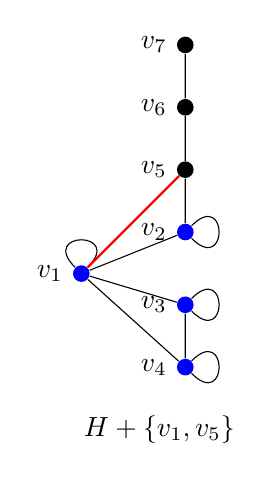
\begin{tikzpicture}[scale=0.66, vertex/.style={minimum width=6pt, circle, inner sep=0pt}]
\node[vertex,fill=blue, label=left:$v_1$](1) at (-1,0){};
\node[vertex,fill=blue, label=left:$v_2$](2) at (1,0.8){};
\node[vertex,fill=blue, label=left:$v_3$](3) at (1,-0.6){};
\node[vertex,fill=blue, label=left:$v_4$](4) at (1,-1.8){};
\node[vertex,fill, label=left:$v_5$](5) at (1,2){};
\node[vertex,fill, label=left:$v_6$](6) at (1,3.2){};
\node[vertex,fill, label=left:$v_7$](7) at (1,4.4){};
\draw (1) to [out=45, in=135, loop, min distance=1cm](1);
\draw (2) to [out=45, in=315, loop, min distance=1cm](2);
\draw (3) to [out=45, in=315, loop, min distance=1cm](3);
\draw (4) to [out=45, in=315, loop, min distance=1cm](4);
\draw(1)--(3)--(4)--(1)--(2)--(5)--(6)--(7);
\draw[red,thick](1)--(5);
\node at (0.5,-3){$H+\{v_1,v_5\}$};
\end{tikzpicture}}

\sbox{\Hthreebox}{%
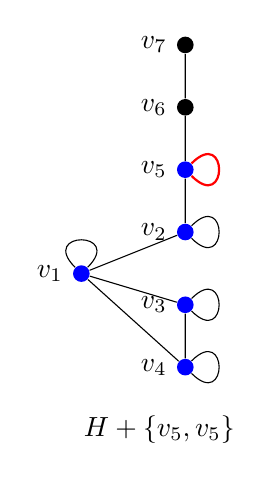
\begin{tikzpicture}[scale=0.66, vertex/.style={minimum width=6pt, circle, inner sep=0pt}]
\node[vertex,fill=blue, label=left:$v_1$](1) at (-1,0){};
\node[vertex,fill=blue, label=left:$v_2$](2) at (1,0.8){};
\node[vertex,fill=blue, label=left:$v_3$](3) at (1,-0.6){};
\node[vertex,fill=blue, label=left:$v_4$](4) at (1,-1.8){};
\node[vertex,fill=blue, label=left:$v_5$](5) at (1,2){};
\node[vertex,fill, label=left:$v_6$](6) at (1,3.2){};
\node[vertex,fill, label=left:$v_7$](7) at (1,4.4){};
\draw (1) to [out=45, in=135, loop, min distance=1cm](1);
\draw (2) to [out=45, in=315, loop, min distance=1cm](2);
\draw (3) to [out=45, in=315, loop, min distance=1cm](3);
\draw (4) to [out=45, in=315, loop, min distance=1cm](4);
\draw[red,thick] (5) to [out=45, in=315, loop, min distance=1cm](5);
\draw(1)--(3)--(4)--(1)--(2)--(5)--(6)--(7);
\node at (0.5,-3){$H+\{v_5,v_5\}$};
\end{tikzpicture}}

\begin{figure}\centering
\begin{minipage}{0.22\textwidth}\centering \visible<1-4>{\usebox{\Hbox}}\end{minipage}\hspace{2pt}
\begin{minipage}{0.22\textwidth}\centering \visible<1-2>{\usebox{\Honebox}}\end{minipage}\hspace{2pt}
\begin{minipage}{0.22\textwidth}\centering \visible<1,3>{\usebox{\Htwobox}}\end{minipage}\hspace{2pt}
\begin{minipage}{0.22\textwidth}\centering \visible<1,4>{\usebox{\Hthreebox}}\end{minipage}
\end{figure}

\medskip
\centering\footnotesize\setlength{\tabcolsep}{4pt}

\only<2>{%
\begin{tabular}{p{0.46\textwidth}|p{0.46\textwidth}}
\hline
\multicolumn{2}{l}{\cellcolor{blue!10}$\lambda=(0.070716, 0.180906, 0.238414, 0.204521, 0.164007, 0.07243, 0.069006)$}\\
\hline
\cellcolor{blue!3}$\mathbb{E}[H,\lambda]=31.218542$ &
\cellcolor{blue!3}$\mathbb{E}[H+\{v_2,v_3\},\lambda]=31.539906$\\
\hline
\end{tabular}
}

\only<3>{%
\begin{tabular}{p{0.46\textwidth}|p{0.46\textwidth}}
\hline
\multicolumn{2}{l}{\cellcolor{blue!10}$\lambda=(0.08502, 0.06418, 0.076071, 0.096493, 0.336406, 0.326572, 0.015258)$}\\
\hline
\cellcolor{blue!3}$\mathbb{E}[H,\lambda]=13.0179$ &
\cellcolor{blue!3}$\mathbb{E}[H_2,\lambda]=13.058815$\\
\hline
\end{tabular}
}

\only<4>{%
\begin{tabular}{p{0.46\textwidth}|p{0.46\textwidth}}
\hline
\multicolumn{2}{l}{\cellcolor{blue!10}$\lambda=(0.104627, 0.052725, 0.194586, 0.190934, 0.117413, 0.225466, 0.114249)$}\\
\hline
\cellcolor{blue!3}$\mathbb{E}[H,\lambda]=33.838547$ &
\cellcolor{blue!3}$\mathbb{E}[H_3,\lambda]=35.972599$\\
\hline
\end{tabular}
}
\end{frame}

\section{Conclusion}
\begin{frame}{Conclusion and Future work}
\begin{fullpageitemize}
\item[-] \textbf{Simple Graphs}
\item Performed simulations for star-free graphs
\item[-] \textbf{Multiple Graphs}
\item Derived the product-form expression for expectation
\item Developed a program for simulation
\item[-] \textbf{Open Problems}
\item No paradox under FCFM for graph with  a loop for all node ?
\item Explore other matching policies for possible paradoxical behavior
\end{fullpageitemize}
\end{frame}

%\framepic[0.8]{images/skeleton}{
%\begin{textblock}{}(10,5)
%{\color{inriared}\hugetext{\textbf{RUN!}}}
%\end{textblock}}

\setbeamercolor{background canvas}{bg=inriagray}

\begin{frame}[plain]
\begin
{center}
\vfill
\color{white}
\Hugetext{Questions?}
\vfill
{\large Gracias ~~~~ Merci ~~~~ Thanks ~~~~ XieXie}
\vfill
\end{center}
\end{frame}

\end{document}